\documentclass[tikz,border=4pt]{standalone}
\usepackage{tikz}
\usepackage{amsmath}
\usepackage{bm}
\usetikzlibrary{arrows.meta,calc,fit,positioning,shapes.geometric,backgrounds}

\begin{document}
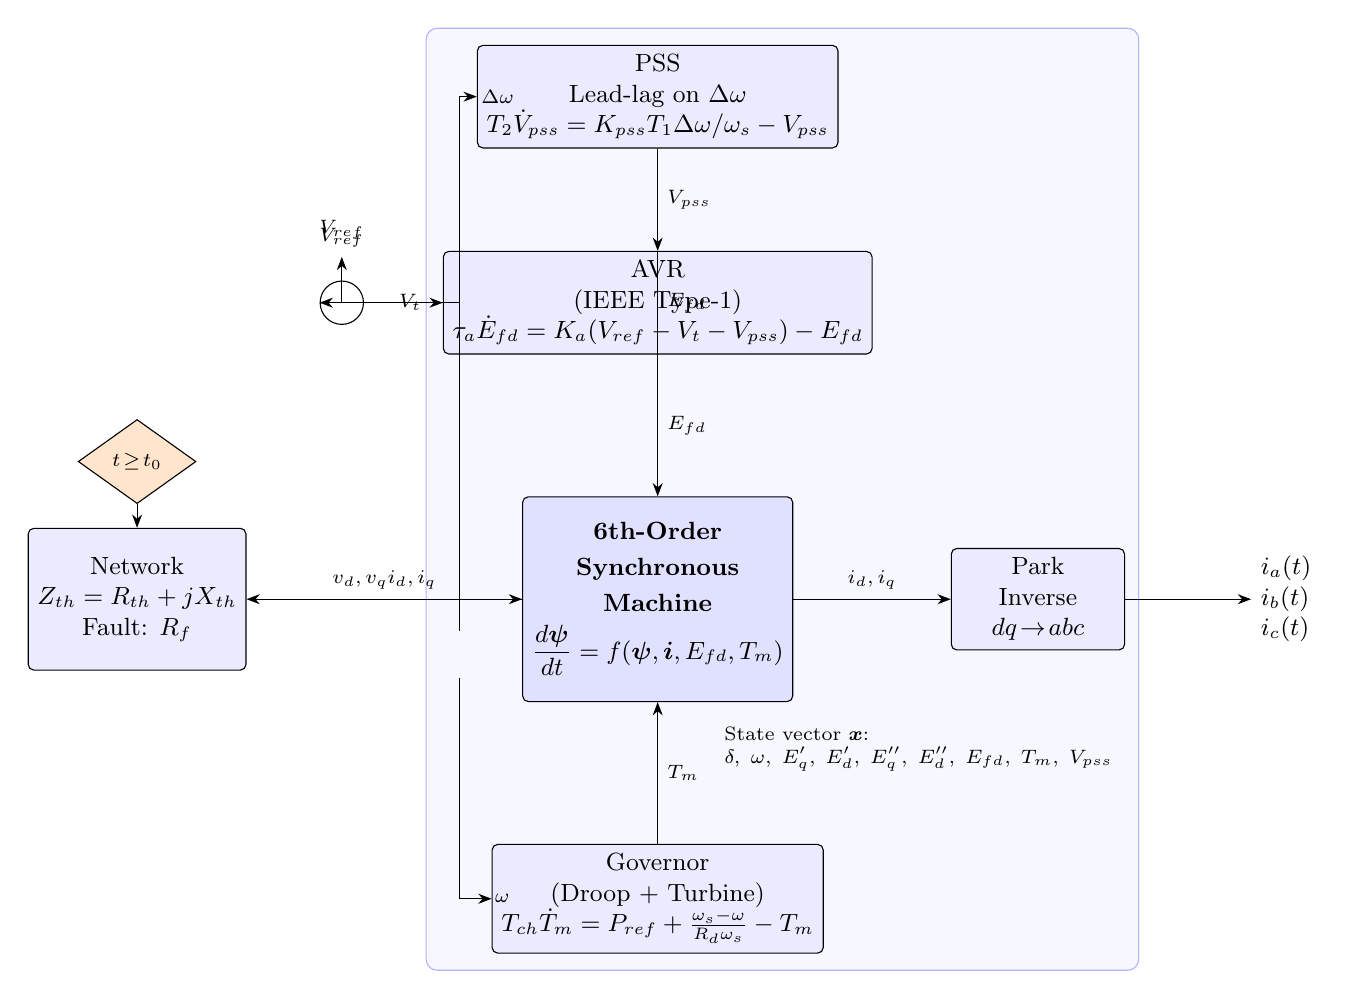
\begin{tikzpicture}[
  font=\small,
  >=Stealth,
  block/.style={draw,rectangle,minimum width=2.2cm,minimum height=0.85cm,
                align=center,fill=blue!8,rounded corners=2pt},
  sum/.style  ={draw,circle,minimum size=0.55cm,inner sep=0pt},
  label/.style={font=\scriptsize},
]

%% ============================================================
%% Columns:  x=0 (inputs), x=3.5 (machine core), x=7.5 (outputs)
%% ============================================================

% --- Machine core (centre) ---
\node[block,minimum width=3.0cm,minimum height=2.6cm,
      fill=blue!12,align=center] (machine) at (4,0)
      {\textbf{6th-Order}\\[2pt]\textbf{Synchronous}\\[2pt]\textbf{Machine}\\[4pt]
       $\dfrac{d\bm{\psi}}{dt} = f(\bm{\psi},\bm{i},E_{fd},T_m)$};

% --- Park transform block (right of machine) ---
\node[block,right=2.0cm of machine] (park)
      {Park\\Inverse\\$dq \!\to\! abc$};

% --- abc output ---
\node[right=1.6cm of park,align=left] (iabc)
      {$i_a(t)$\\$i_b(t)$\\$i_c(t)$};

\draw[->] (machine.east) -- node[above,label]{$i_d,i_q$} (park.west);
\draw[->] (park.east)    -- (iabc.west);

% --- AVR block (above machine) ---
\node[block,above=1.8cm of machine] (avr)
      {AVR\\(IEEE Type-1)\\$\tau_a\dot{E}_{fd}=K_a(V_{ref}-V_t-V_{pss})-E_{fd}$};

\node[sum,left=1.0cm of avr] (savr) {};
\node[above=0.4cm of savr,label] {$V_{ref}$};
\draw[->] (savr.north) -- ++(0,0.3) node[label,above]{$V_{ref}$};

% --- PSS block (above AVR) ---
\node[block,above=1.3cm of avr] (pss)
      {PSS\\Lead-lag on $\Delta\omega$\\$T_2\dot{V}_{pss}=K_{pss}T_1\Delta\omega/\omega_s - V_{pss}$};

\draw[->] (avr.north) -- node[right,label]{$E_{fd}$} (machine.north|-avr.south)
          -- node[right,label]{$E_{fd}$} (machine.north);
\draw[->] (pss.south) -- node[right,label]{$V_{pss}$} (avr.north);

% --- Vt feedback ---
\draw[->] (machine.west) -- ++(-0.8,0) |- node[pos=0.75,right,label]{$V_t$}
          (savr.west);
\draw[->] (savr.north) |- (avr.west);

% --- Omega feedback to PSS ---
\coordinate (omegaout) at ($(machine.west)+(-0.8,-0.4)$);
\draw[->] (omegaout) |- node[pos=0.85,right,label]{$\Delta\omega$} (pss.west);

% --- Governor block (below machine) ---
\node[block,below=1.8cm of machine] (gov)
      {Governor\\(Droop + Turbine)\\$T_{ch}\dot{T}_m = P_{ref}+\tfrac{\omega_s-\omega}{R_d\omega_s}-T_m$};

\draw[->] (gov.north) -- node[right,label]{$T_m$} (machine.south);

% --- Omega feedback to governor ---
\coordinate (omegagov) at ($(machine.west)+(-0.8,-1.0)$);
\draw[->] (omegagov) |- node[pos=0.9,right,label]{$\omega$} (gov.west);

% --- Network / fault block (left) ---
\node[block,left=3.5cm of machine,minimum height=1.8cm] (net)
      {Network\\$Z_{th}=R_{th}+jX_{th}$\\Fault: $R_f$};

\draw[<->] (net.east) -- node[above,label]{$v_d,v_q$\\$i_d,i_q$} (machine.west);

% --- Fault switch ---
\node[draw,diamond,aspect=1.4,minimum size=0.6cm,fill=orange!20,
      above=0.3cm of net,font=\scriptsize] (sw) {$t\!\geq\!t_0$};
\draw[->] (sw) -- (net);

% --- Title and state vector annotation ---
\node[align=left,font=\scriptsize,below right=0.2cm and -1.0cm of machine]
  (sv) {State vector $\bm{x}$:\\
        $\delta,\;\omega,\;E'_q,\;E'_d,\;E''_q,\;E''_d,\;E_{fd},\;T_m,\;V_{pss}$};

\begin{scope}[on background layer]
  \node[draw=blue!30,fill=blue!3,rounded corners=4pt,
        fit=(machine)(avr)(pss)(gov)(sv),inner sep=6pt] {};
\end{scope}

\end{tikzpicture}
\end{document}
